% Addendum to sec:ml, staged for the margins revision.  Two
% paragraphs: the finite-size/algorithmic measurement the section
% calls for, and the multi-state prior comparison.  Wire into main.tex
% at the end of sec:ml when the margins set closes.

The algorithmic gap the curve frames is directly measurable at
moderate size.  A population annealer (hinge energy on violated
margins, geometric schedule matched to the $2/\sqrt N$ energy scale;
\texttt{finite\_size\_experi\-ment.py}) trained $N=101$ instances across
$\alpha$ at $\kappa\in\{0,0.05,0.1\}$.  Its success walls (the half-success crossings) fall in the correct
$\kappa$ order and sit below the corresponding
$\alpha_\star(\kappa)$ by $0.08$--$0.12$ in $\alpha$ at this budget,
while scattered successes persist to the bound itself: at
$\kappa=0.1$ the last appear at $\alpha\approx0.73$, essentially at
$\alpha_\star$, and none beyond.  The solutions the
annealer does find are atypical in exactly the direction the
clustering picture predicts: at low load their mean gap above
$\kappa$ tracks the typical-solution law $p(h)$, while near the wall
it holds around $0.65$--$0.70$ as the typical mean descends --- the
algorithm reaches the wide, over-margined minority.  At $N=201$ under the same
per-spin budget the walls sharpen and shift left, so what the
annealer traces is a budget-dependent lower envelope of the true
algorithmic threshold, whose location and the clustering barrier
behind it are the subject of a substantial
literature~\cite{gamarnik2022algorithms,lsz2024} on the closely
related symmetric and asymmetric binary perceptrons; the
found-solution histograms meanwhile track
the derived $p(h)$ closely at moderate load and deform toward
mid-gaps near the wall.  Both effects are schedule-dependent
observations, not thresholds; the certified curve is what they are
measured against, and the comparison compresses neatly: within each
size and budget the wall sits at a $\kappa$-independent fraction of
$\alpha_\star(\kappa)$ ($0.90$ at $N=101$ down to $0.50$ at $N=801$,
flat across margins to better than one percent at the largest
sizes), so the demanded
margin costs the algorithm the same relative capacity it costs the
storage bound (Figure~\ref{fig:fraction}).  At fixed sweeps per spin
the fraction falls with $N$ --- $0.90$, $0.75$, $0.69$, $0.63$,
$0.50$ at $N=101$, $201$, $301$, $401$, $801$ --- close to a fixed
loss of $0.13$ per doubling over the measured range, so an early
$1/N$ reading of the first three sizes (which would have leveled
near $0.59$) is refuted by the larger ones; holding a constant
fraction of capacity requires superlinearly growing total work.  On
the budget axis at $N=201$ the fraction climbs $0.75$, $0.79$,
$0.86$ as the budget quadruples twice, but a further quadrupling to
$25{,}600$ sweeps per spin gains only $0.02$ ($0.876$): the fixed
gain per quadrupling stops at $6{,}400$, and the wall saturates near
$0.88$ of capacity at this size over the measured range.

\begin{figure}[t]
\centering
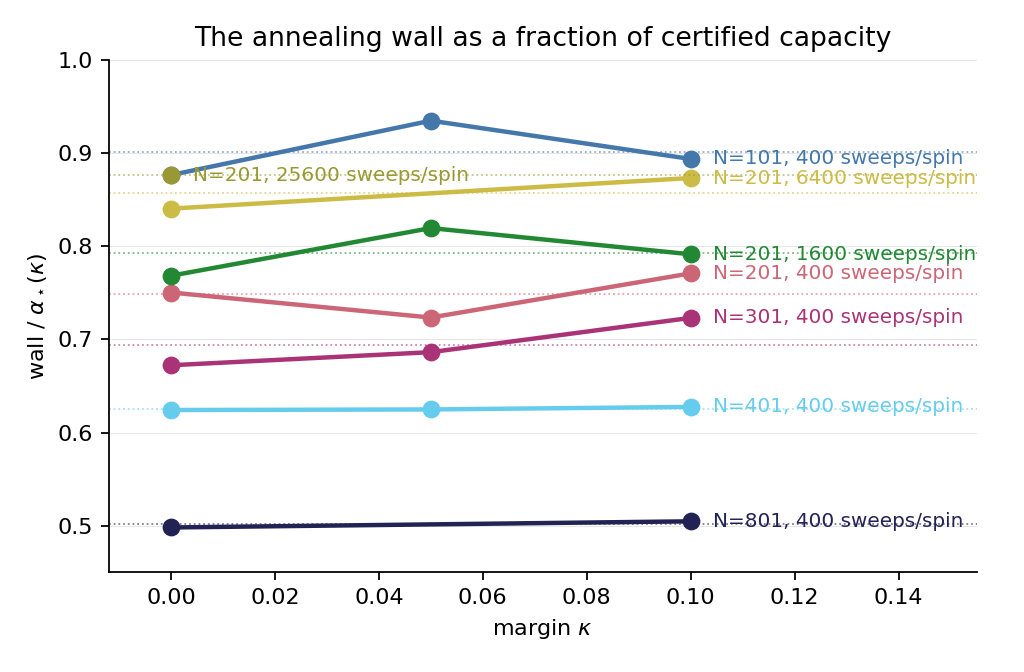
\includegraphics[width=0.8\linewidth]{algorithmic_fraction.png}
\caption{The annealing wall as a fraction of the certified capacity
$\alpha_\star(\kappa)$, across size--budget pairs.  Within each
run the fraction is flat in $\kappa$ to a few percent, while its
level depends on both size and budget.}
\label{fig:fraction}
\end{figure}

The margin price also depends on the weight alphabet.  Solving the
replica-symmetric system for ternary weights $\{-1,0,+1\}$ with a
self-overlap order parameter (\texttt{exploration/\allowbreak ternary\_km.py},
anchored by reproducing the binary $\alpha_\star(0)=0.8330786$ to the
certified digits) gives $\alpha_\star^{\mathrm{tern}}(0)=1.17448$
against an annealed bound of $\log_2 3$, with $1.07951$ at
$\kappa=0.05$ and $0.99483$ at $\kappa=0.1$.  Per weight \emph{state} the richer alphabet stores
more; per weight \emph{bit} it stores less --- $0.741$ against the
binary $0.833$ constraints per bit at $\kappa=0$, and the gap widens
monotonically with margin ($0.100$ at $\kappa=0.05$, $0.105$ at $0.1$).  At this level of the theory,
binary remains the bit-efficient quantization for robust storage.  The full eight-point curve (Figure~\ref{fig:ternary},
$\kappa$ up to $0.35$) makes this a statement about the whole margin
range rather than three samples: per stored bit the binary curve sits
above the ternary one everywhere, the absolute gap saturating near
$0.11$ constraints per bit above $\kappa\approx 0.2$ while the
relative advantage grows from $12$ to $26$ percent, since both
capacities fall with margin.

\begin{figure}[t]
\centering
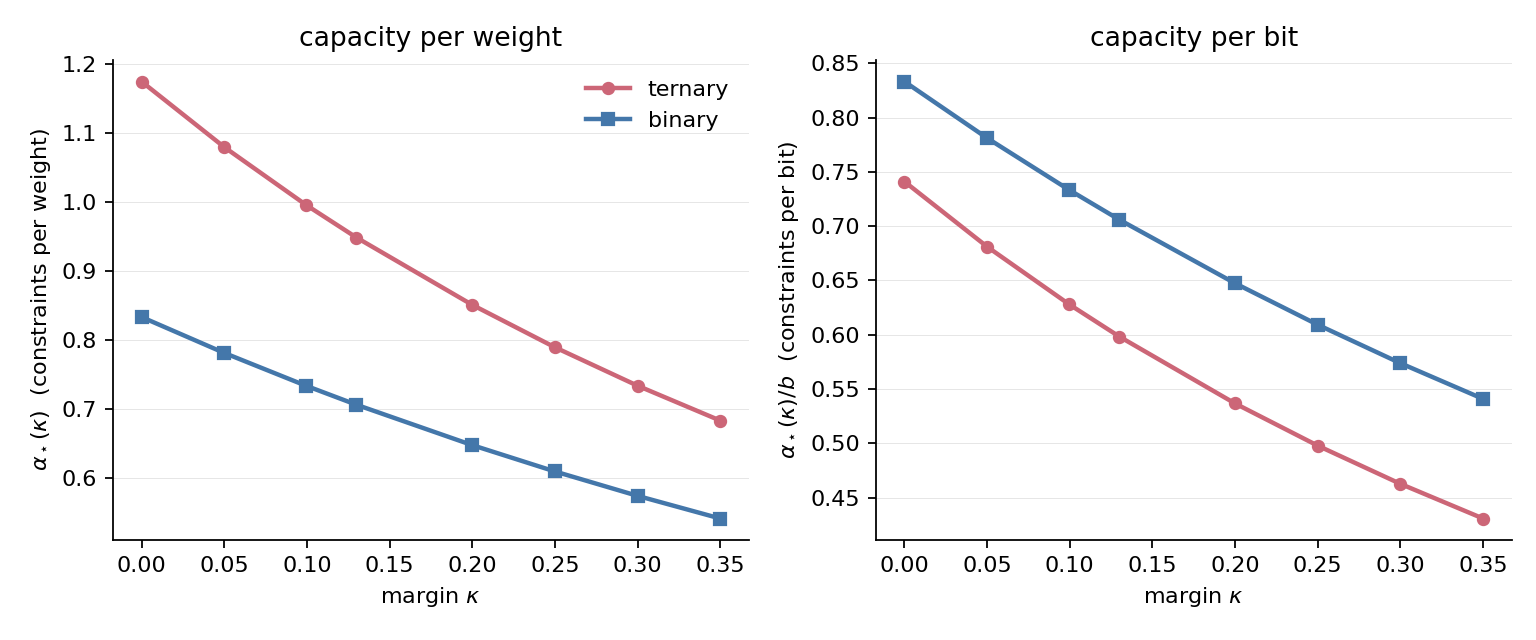
\includegraphics[width=0.98\linewidth]{ternary_comparison.png}
\caption{Replica-symmetric capacity of ternary against binary
weights, per weight (left) and per stored bit (right, dividing by
$\log_2 3$ and $1$).  The order reverses: the richer prior stores
more per weight and less per bit, at every computed margin.}
\label{fig:ternary}
\end{figure}
